% =====================================================================
%  合订本 —— 研究报告 + 佐证材料（附录），单文件提交用
%  编译：先确保 main.pdf 与 evidence.pdf 已生成，再 xelatex combined.tex
% =====================================================================
\documentclass[a4paper,12pt,fontset=none]{ctexart}
\usepackage[a4paper,margin=2.5cm]{geometry}
\setCJKmainfont{Noto Serif CJK SC}
\setCJKsansfont{Noto Sans CJK SC}
\usepackage{pdfpages}
\usepackage{tikz}
\usepackage{xcolor}
\definecolor{abbred}{RGB}{217,74,31}
\definecolor{abbdark}{RGB}{24,24,24}
\definecolor{abbgray}{RGB}{95,95,95}
\definecolor{abblight}{RGB}{246,242,240}
\pagestyle{empty}

\begin{document}

% ---- 第一部分：项目研究报告（含其自带封面）----
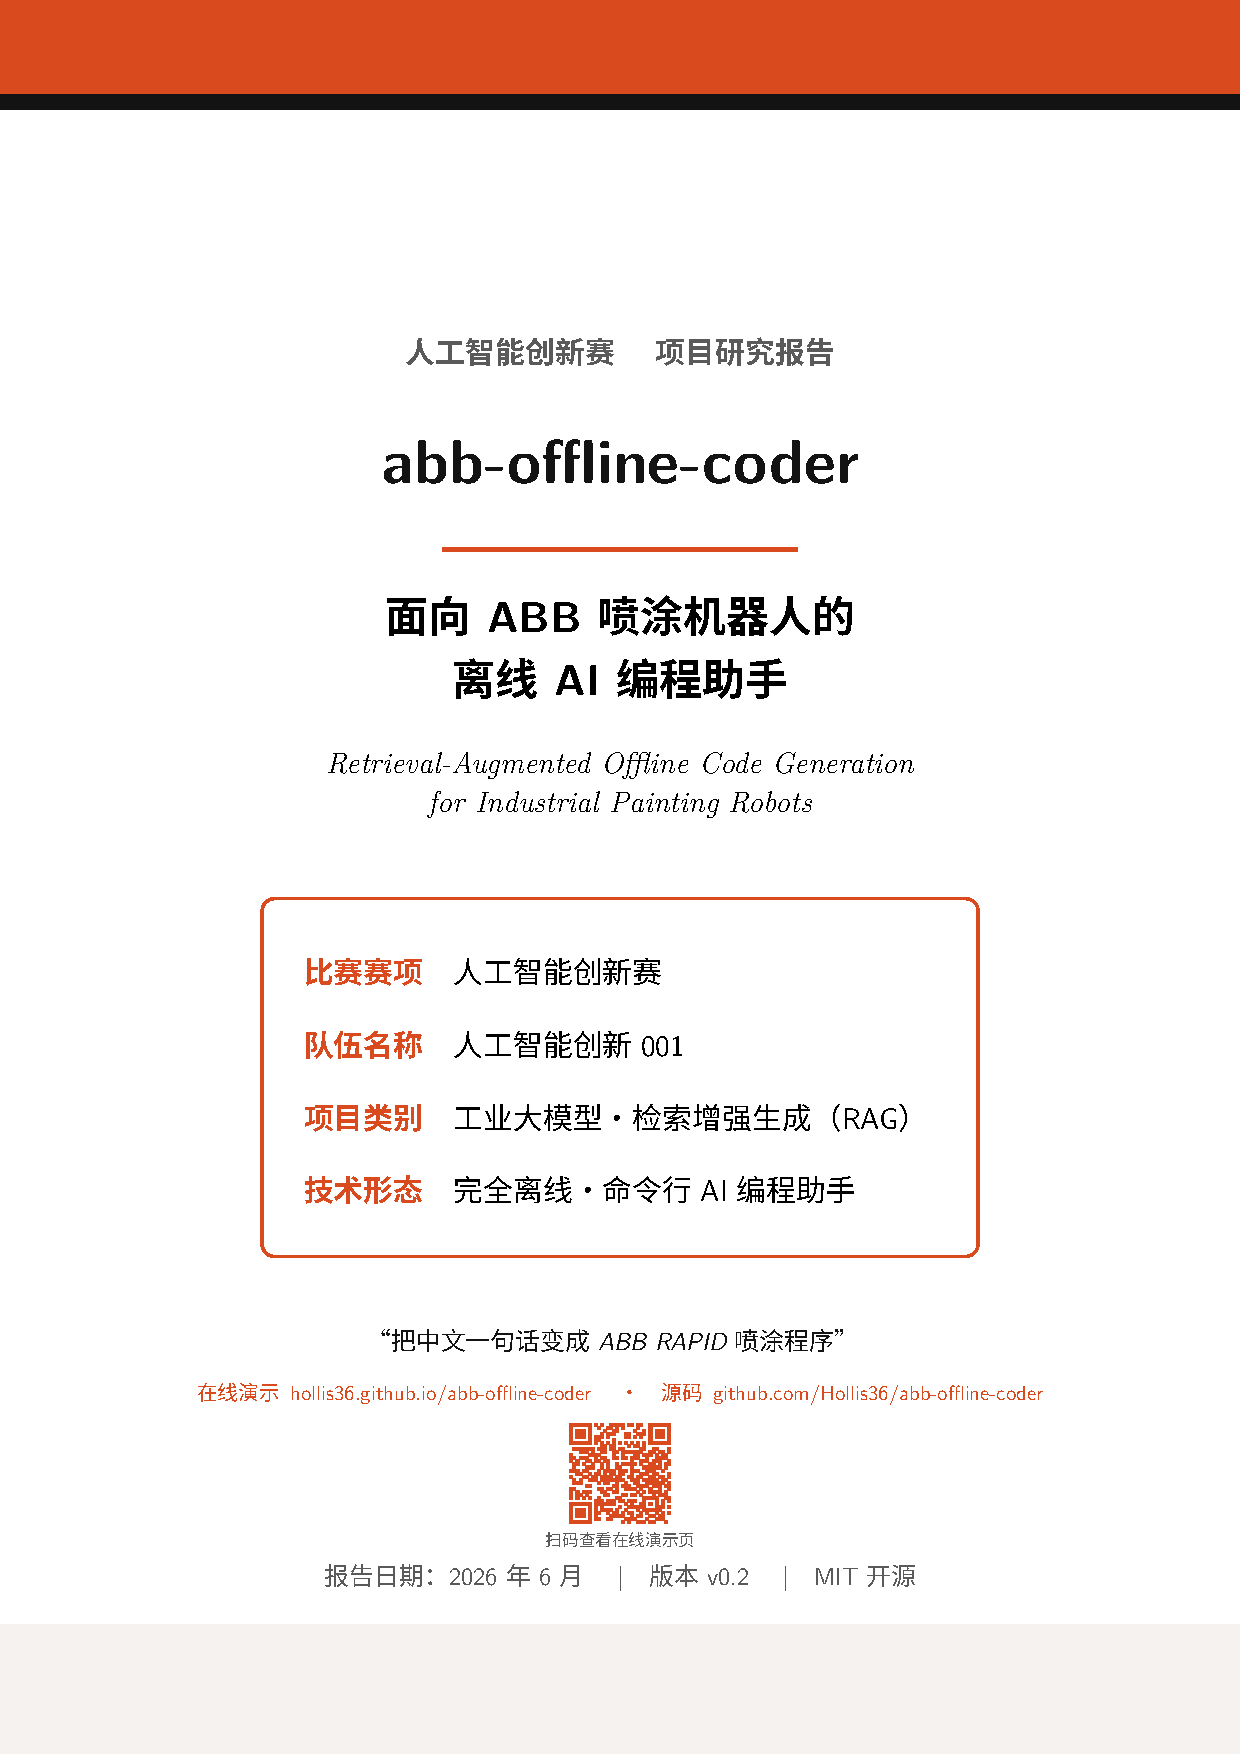
\includepdf[pages=-,fitpaper=true]{main.pdf}

% ---- 附录分隔页 ----
\thispagestyle{empty}

\begin{tikzpicture}[remember picture,overlay]
  \fill[abbred] (current page.north west) rectangle ([yshift=-1.6cm]current page.north east);
  \fill[abbdark] ([yshift=-1.6cm]current page.north west) rectangle ([yshift=-1.85cm]current page.north east);
  \fill[abblight] (current page.south west) rectangle ([yshift=2.2cm]current page.south east);
\end{tikzpicture}
\vspace*{6cm}
\begin{center}
{\sffamily\bfseries\color{abbgray}\Large 人工智能创新赛 · abb-offline-coder}\\[1.4cm]
{\sffamily\fontsize{40}{46}\selectfont\bfseries\color{abbdark} 附\quad 录}\\[0.5cm]
{\color{abbred}\rule{6cm}{2pt}}\\[0.7cm]
{\sffamily\LARGE\bfseries 项目佐证材料}\\[0.4cm]
{\large\color{abbgray} 可复现实测 · Git 历史 · 单元测试 · 核心能力实跑 · 真实产物 · 公开发布物料}
\end{center}
\vfill
\begin{center}{\sffamily\small\color{abbgray}
队伍：人工智能创新001 \quad|\quad 完全离线 · 中文需求 → ABB RAPID 喷涂程序}\end{center}
\clearpage

% ---- 第二部分：项目佐证材料 ----
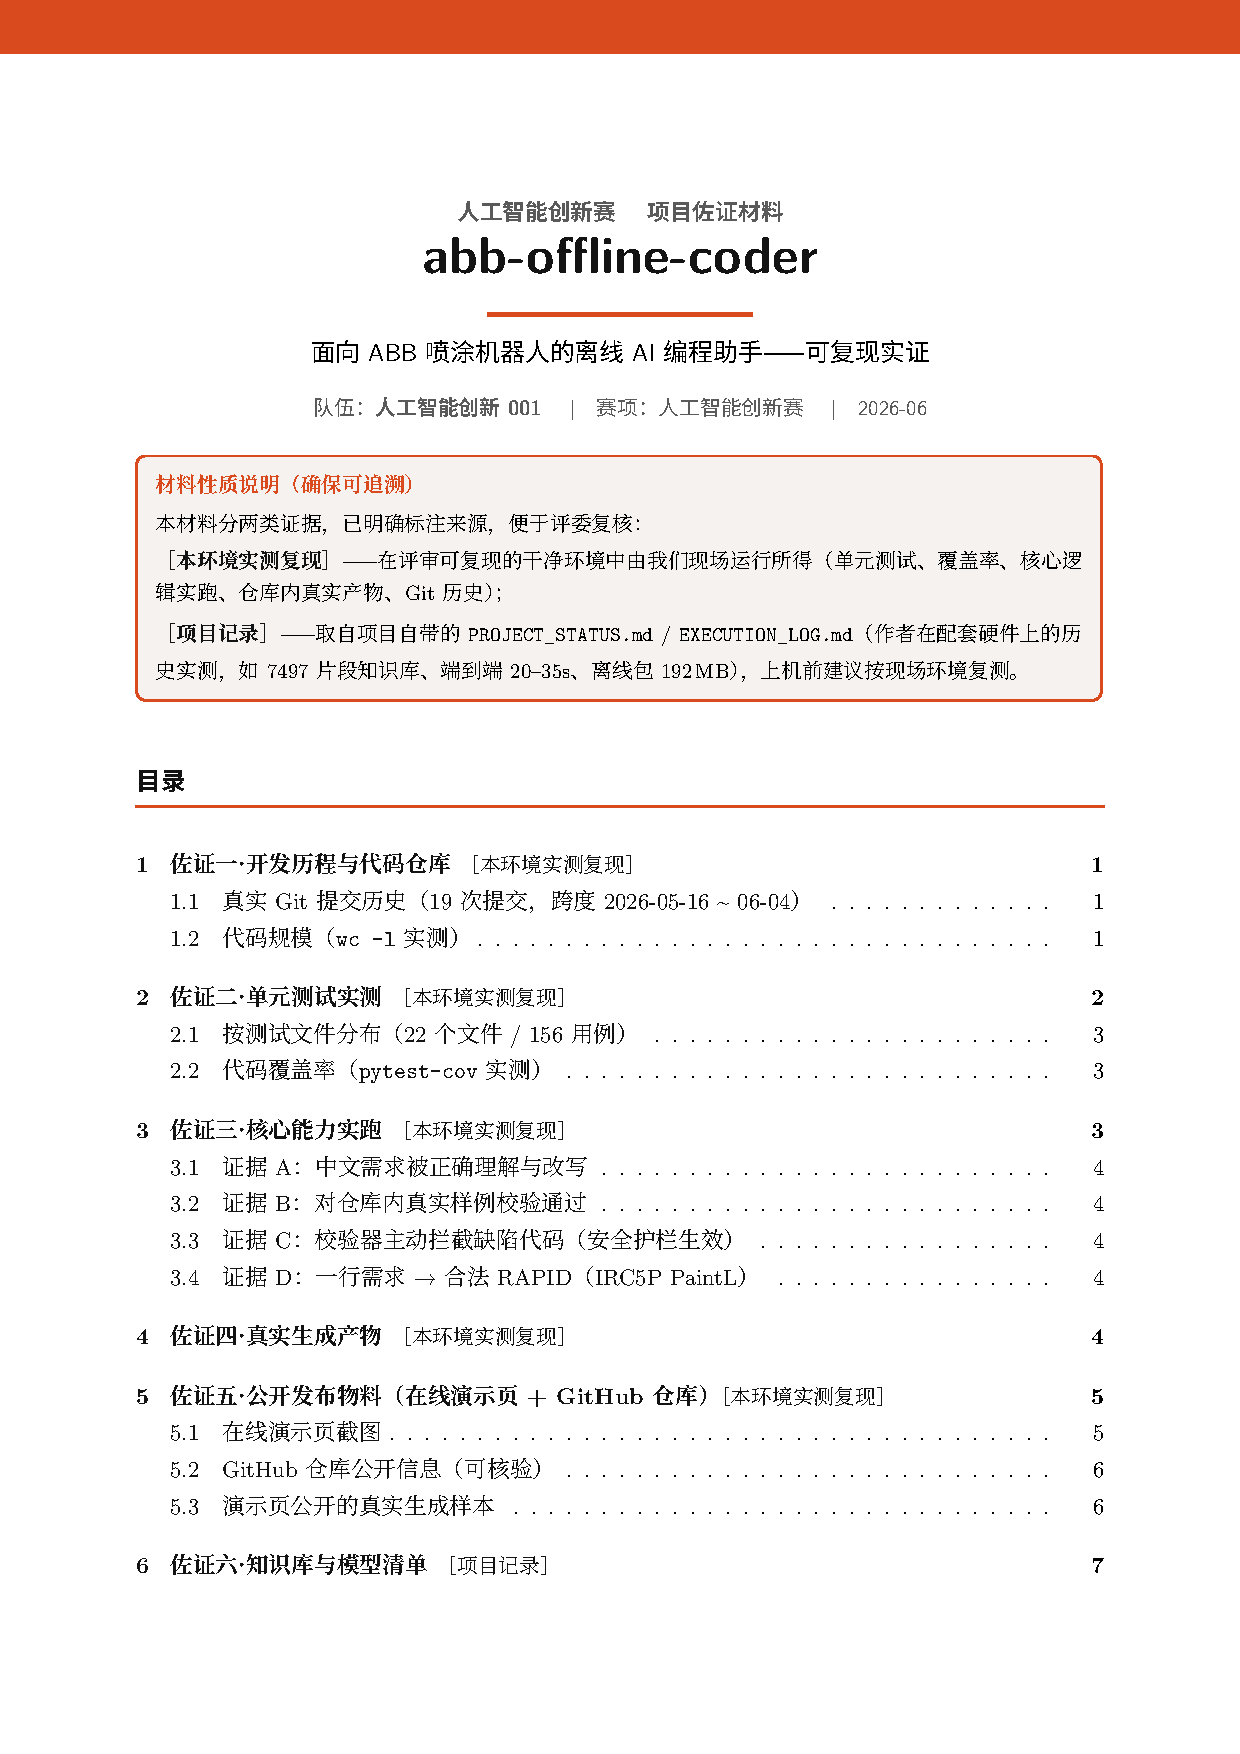
\includepdf[pages=-,fitpaper=true]{evidence.pdf}

\end{document}
